\section{ProgCPP}

    \subsection{Nützliche Links}
        \begin{itemize}
            \item STL: https://en.cppreference.com/
            \item Boost: https://www.boost.org/
            \item Github (Lizenzen beachten!)
        \end{itemize}

    \subsection{Wichtige Kurzbefehle}
        \begin{tabular}{ll}
            \verb|cd "Path"| & Pfad anwählen \\
            \verb|cd ..| & um eine Ebene nach oben (zurück) \\
            \verb|mkdir "Ordnername"| & Ordner erstellen \\
            \verb|rmkdir "Ordnername"| & Ordner löschen \\
            \verb|rm -rf *| & Alles innerhalb vom aktuellen Ordner löschen \\
            \verb|rm "Datei"| & Datei löschen \\
            \verb|mv "Name alt" "Name neu"| & Datei umbenennen \\
            \verb|cp "Datei alt" "Datei neu"| & Datei kopieren und benennen \\
            \verb|clang++ -Wall -o "Outputname" "Inputdatei"| & clang++ - Compiler mit Warnungen \\
            %\verb|clang++ -Wall -o "Outputname" "Inputdatei" -lm| & -lm für Mathebibliothek \\
            \verb|ls| & Listet alle Files im akt. Verzeichnis auf \\
            \verb|ls -l| & Inkl. Informationen wie Grösse u.a. \\
            \verb|ls -a| & Inkl. versteckten Dateien \\
            \verb|ls -al| & Beide Varianten \\
        \end{tabular}

    \subsection{Datentypen}

        \subsubsection{Namen}
            \begin{tabular}{|l|l|l|}
                \hline
                Variablen, Konstanten & Funktionen & Klassen, Strukt., Enums \\
                \hline
                mit Kleinbuchst. beginnen & mit Kleinbuchst. beginnen & mit Grossbuchst. beginnen \\
                camelCase & camelCase & PascalCase \\
                keine Underscores & keine Underscores & keine Underscores \\
                &&\\
                \verb|maxSpeed| & \verb|getCount()| & \verb|MotorController| \\
                \hline
            \end{tabular}

    \subsection{Streams}
        Ein Stream rep. einen Datenstrom, z.B. ein Terminal, Dateien oder Datenverkehr (TCP/IP).

        \textbf{Standardströme:}
        \begin{itemize}
            \item \verb|cin|
            \item \verb|cout|
            \item \verb|cerr|
            \item \verb|clog|
        \end{itemize}

        \verb|cin| und \verb|cout| müssen ganz links in der Zeile stehen!

        \subsubsection{Flags}
            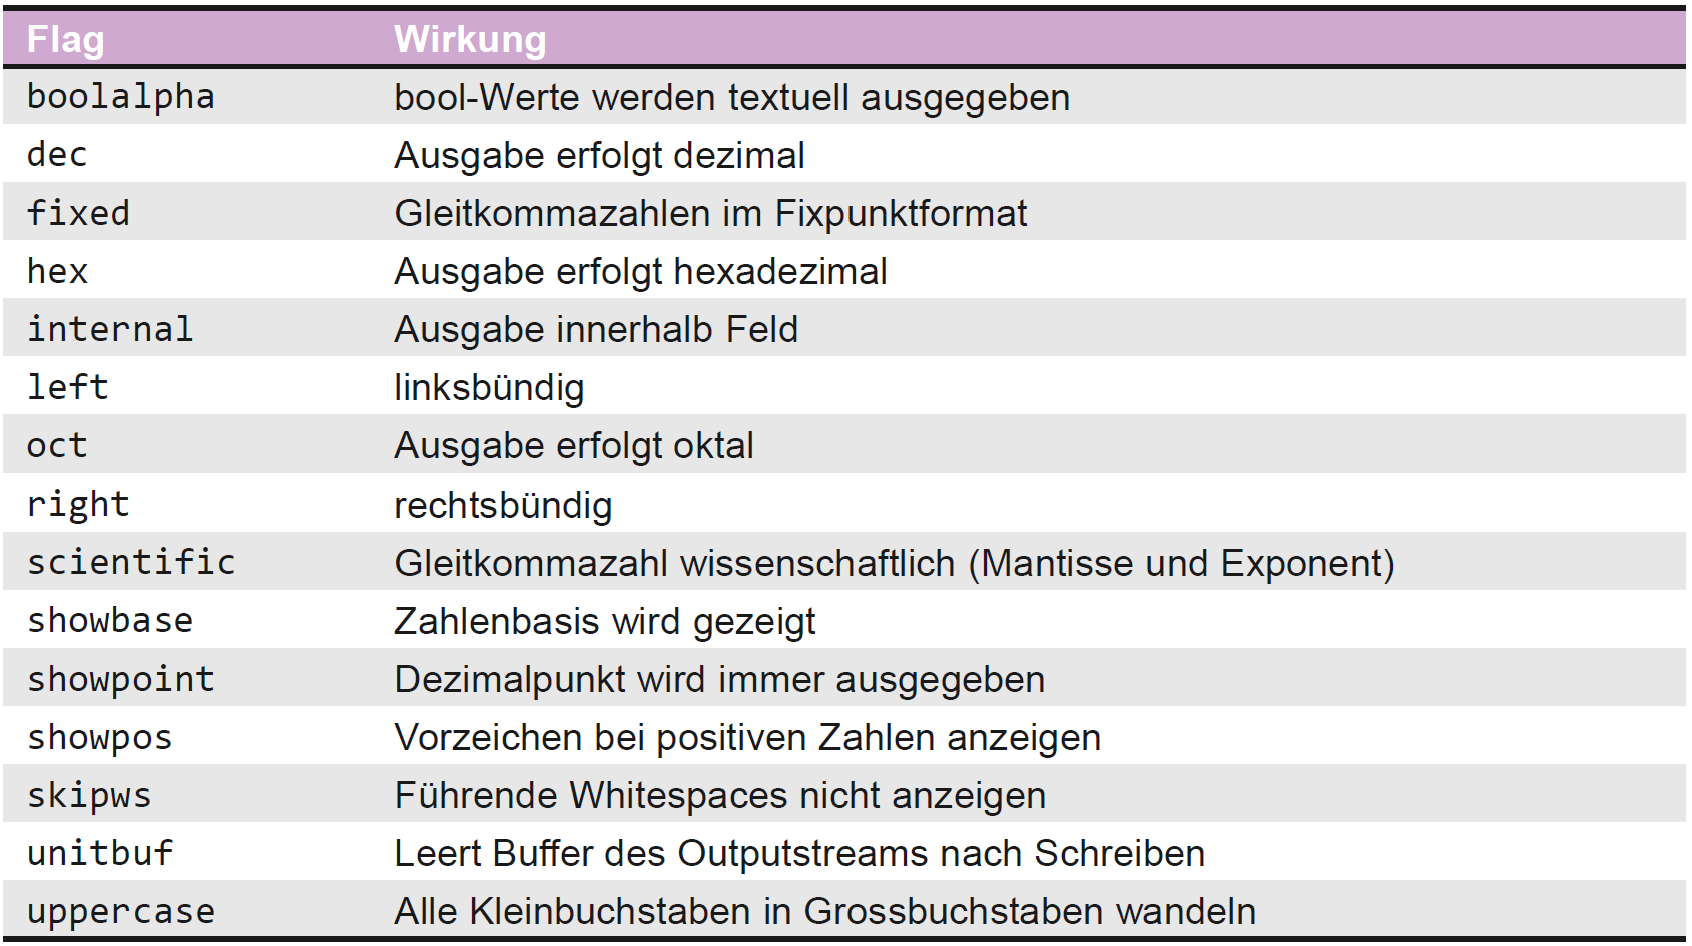
\includegraphics[width=0.95\linewidth]{Bilder/cpp_flags-iostream.png}

    \subsection{Klassen, Methoden und Objekte}
        Objekte verfügen über Attribute, Methoden und eine Identität.

        Ähnliche Objekte werden in Klassen zusammengefasst.

        Klassen können auch mit \verb|struct| definiert werden. \verb|struct| definiert alles \textbf{public}, \verb|class| alles \textbf{private}

        \subsubsection{Klassen}
            Bsp: \verb|drink.h| \\ %UML-Generator: https://app.smartdraw.com/editor.aspx?templateId=3f94c5ba-46fb-46ac-80e2-8b13581b08db&flags=128#depoId=55119816&credID=-60756356
            \begin{minipage}{0.45\linewidth}
                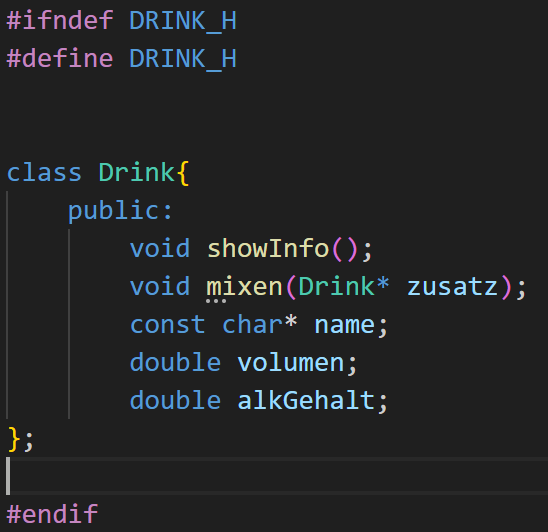
\includegraphics[width=0.95\linewidth]{Bilder/cpp_klassen-hfile-bsp.png}
            \end{minipage}
            \hfill
            \begin{minipage}{0.3\linewidth}
                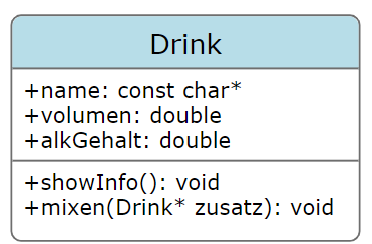
\includegraphics[width=0.95\linewidth]{Bilder/cpp_klassen-hfile-uml.png}
            \end{minipage}
            \begin{minipage}{0.2\linewidth}
                \begin{itemize}
                    \item + public
                    \item - private
                    \item \verb|#| protected
                \end{itemize}
            \end{minipage}
            
            Inkl. Include-Guard für das h-File, nebenan das UML-Diagramm

        \subsubsection{Methoden}
            Bsp: \verb|drink.cpp| \\
            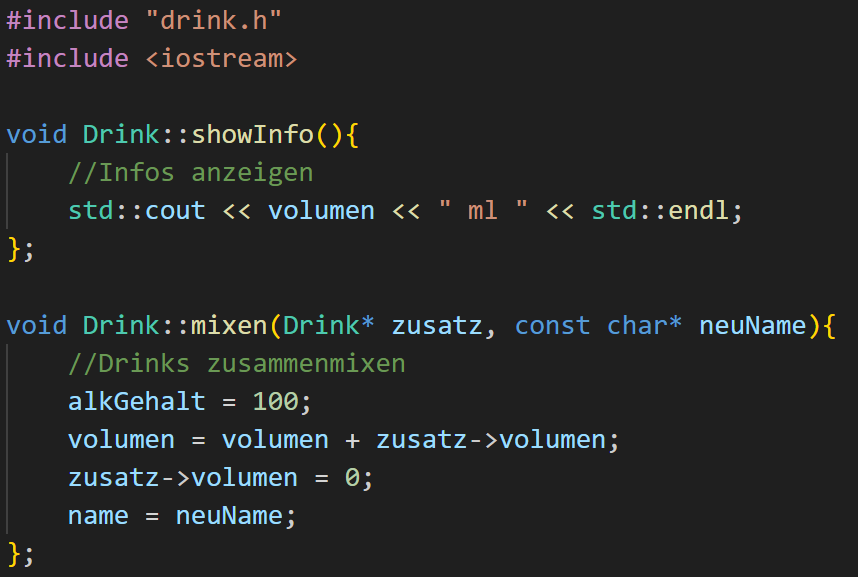
\includegraphics[width=0.7\linewidth]{Bilder/cpp_klassen-hfile-methoden.png}
            
            \textit{Wichtig:} h-Files werden mit $".."$ eingegliedert
            \\
            \textbf{Objekte}
            
            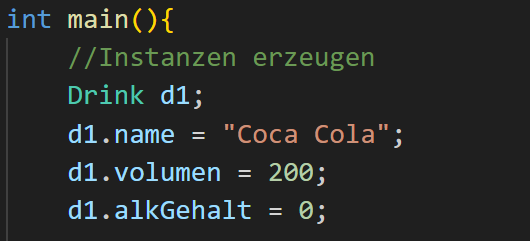
\includegraphics[width=0.7\linewidth]{Bilder/cpp_klassen-objekte.png}

    \subsection{Make}
        \verb|Make| dient als Tool, um Compilerdurchläufe zu optimieren.
        Das Tool kompiliert nur Files neu, welche seit dem letzten Durchlauf geändert wurden.

        Sofern nicht anders angegeben, beginnt \verb|make| mit dem obersten Befehl.

        \begin{minipage}{0.5\linewidth}
            \textbf{Makefile}
            \begin{lstlisting}[language=C++]
#Variablen
CXX = clang++
CXXFLAGS = -Wall -c
LDFLAGS = -o
BIN = vektor3d
OBJS = vektor3d.o main.o

all: $(BIN)

#Alle .cpp in .o wandeln
%.o: %.cpp
	$(CXX) $(CXXFLAGS) $<

$(BIN): $(OBJS)
	$(CXX) $(LDFLAGS) $@ $^

clean:
	rm -f $(BIN) $(OBJS) vektor3d.exe

.PHONY: clean all
            \end{lstlisting}
        \end{minipage}
        \hfill
        \begin{minipage}{0.45\linewidth}
            \textbf{Befehle}:\\
            \verb|<Target>: <Dependency1> <Dependency2> ...|\\
            \textbf{Platzhalter}
            \begin{itemize}
                \item \verb|$@|: Dateiname des Targets
                \item \verb|$^|: Dateiname aller Dependencies
                \item \verb|$<|: Dateiname der ersten Dependency
                \item \verb|#| : Für Kommentare
                \item \verb|%| : Für beliebiges Target
            \end{itemize}

            Phony dient zur Kennzeichnung von Befehlen ohne Output
        \end{minipage}



    \subsection{Operatoren und Operanden}

        \subsubsection{Logisch vs. bitweise Operatoren}
            $\parallel$ oder \verb|'or'| = OR\\
            \&\& oder \verb|'and'| = AND \\
            \\
            \textbf{Logisch:}
                \begin{lstlisting}[language=C++]
char a = 0;   //bedeutet unwahr
char b = -27; //bedeutet wahr
if(a and b){
cout << "A und B sind wahr" << endl;
}	
                \end{lstlisting}

    \subsection{Code-Snippets}

        \subsubsection{Hello World!}
            \begin{lstlisting}[language=C++]
#include <iostream>
using namespace std;

int main(){
    cout << "Hello World!" << endl;
    return 0;
}
            \end{lstlisting}
